\documentclass[11pt]{article}
\usepackage[margin=1in]{geometry}
\usepackage{amsmath,amssymb,amsthm}
\usepackage{booktabs}
\usepackage{graphicx}
\usepackage{xcolor}
\usepackage{tikz}
\usetikzlibrary{arrows.meta,positioning,calc,fit}
\usepackage[hidelinks]{hyperref}
\usepackage{caption}
\usepackage{parskip}
\usepackage{float}
\usepackage{tabularx}
\usepackage{url}

% auto-generated by train/report_numbers.py
\newcommand{\RefLoss}{3.295}
\newcommand{\UniCE}{7.649}
\newcommand{\RefFour}{3.204}
\newcommand{\UniFour}{7.631}
\newcommand{\BaseFour}{3.191}
\newcommand{\OneTwenty}{7.652}
\newcommand{\TwoTwenty}{7.652}
\newcommand{\OneFour}{7.632}
\newcommand{\TwoFour}{7.631}
\newcommand{\BaseFinal}{3.312}
\newcommand{\BaseLast}{3.312}
\newcommand{\BaseStop}{4768}
\newcommand{\BaseTokens}{2.50B}
\newcommand{\BasePlateau}{3.801}
\newcommand{\BaseKL}{4.3565}
\newcommand{\BaseGrowth}{1.1}
\newcommand{\BaseGrowthInit}{1.10}
\newcommand{\BaseNormEnd}{44}
\newcommand{\OneFinal}{--}
\newcommand{\OneLast}{7.628}
\newcommand{\OneStop}{3951}
\newcommand{\OneTokens}{2.07B}
\newcommand{\OnePlateau}{7.651}
\newcommand{\OneKL}{0.0046}
\newcommand{\OneGrowth}{18.3}
\newcommand{\OneGrowthInit}{1.15}
\newcommand{\OneNormEnd}{$2.6\times10^{17}$}
\newcommand{\TwoFinal}{--}
\newcommand{\TwoLast}{7.629}
\newcommand{\TwoStop}{3741}
\newcommand{\TwoTokens}{1.96B}
\newcommand{\TwoPlateau}{7.655}
\newcommand{\TwoKL}{0.0042}
\newcommand{\TwoGrowth}{1.6}
\newcommand{\TwoGrowthInit}{1.00}
\newcommand{\TwoNormEnd}{5203}
\newcommand{\ValTable}{0 & 0.00B & 10.957 & 11.012 & 11.005 \\
250 & 0.13B & 5.741 & 7.665 & 7.665 \\
500 & 0.26B & 4.733 & 7.642 & 7.642 \\
1000 & 0.52B & 3.871 & 7.649 & 7.647 \\
1500 & 0.79B & 3.602 & 7.644 & 7.643 \\
2000 & 1.05B & 3.465 & 7.632 & 7.632 \\
2500 & 1.31B & 3.375 & 7.633 & 7.633 \\
3000 & 1.57B & 3.312 & 7.632 & 7.631 \\
3500 & 1.84B & 3.254 & 7.629 & 7.629 \\
4000 & 2.10B & 3.222 & -- & -- \\
4500 & 2.36B & 3.200 & -- & -- \\
\midrule
4768 (final, 20M val) & 2.50B & 3.312 & -- & -- \\}


\newcommand{\code}[1]{\texttt{#1}}
\definecolor{cbase}{HTML}{2a78d6}
\definecolor{cone}{HTML}{eb6834}
\definecolor{ctwo}{HTML}{1baf7a}
\definecolor{ink2}{HTML}{52514e}
\newcommand{\chg}[1]{\colorbox{orange!15}{$\displaystyle #1$}}
\newtheorem{prop}{Proposition}

\title{Training GPT-2 124M from Scratch with Head-wise Attention Residuals:\\
Approach 1 and Approach 2 Collapse to a Unigram Model}
\author{Experiment log, branch \code{attention-experiments}}
\date{2026-10-15}

\begin{document}
\maketitle

\section*{Summary}
We trained three GPT-2 124M models from scratch with identical data, budget and hyperparameters
(Chinchilla-optimal, 2.5B FineWeb-Edu tokens): the standard GPT-2 \textbf{baseline}, and the two
head-wise attention-residual variants \textbf{approach\_1} and \textbf{approach\_2}. The pretrained
OpenAI GPT-2 124M is evaluated on the same validation split for reference.

\begin{center}\small
\begin{tabular}{lrrrl}
\toprule
Model (all trained from scratch & Tokens & \multicolumn{2}{c}{Val loss} & Status \\
\quad except the references) & & 20M split & 4.2M subset & \\
\midrule
\textcolor{cbase}{\textbf{baseline}} (standard GPT-2) & \BaseTokens & \textbf{\BaseFinal} & \BaseFour & completed \\
\textcolor{cone}{\textbf{approach\_1}} & \OneTokens & \OneTwenty & \OneFour & collapsed; stopped, step \OneStop \\
\textcolor{ctwo}{\textbf{approach\_2}} & \TwoTokens & \TwoTwenty & \TwoFour & collapsed; stopped, step \TwoStop \\
OpenAI GPT-2 124M (pretrained) & -- & \RefLoss & \RefFour & reference \\
Unigram (no context) & -- & \UniCE & \UniFour & reference \\
\bottomrule
\end{tabular}
\end{center}
All models are scored on the same tokens in each column. The 4.2M subset (the first 4{,}194{,}304
validation tokens) is what the per-250-step curve points use. The approaches are scored at their last
checkpoint (step 3000).

\textbf{Main finding.} Both approaches reach a loss of $\approx 7.64$ within $\sim$150 steps and never
leave it. That value is the cross-entropy of the \emph{unigram} distribution: on both validation
subsets the approaches match the unigram model to within 0.003 nats (\OneTwenty{} vs.\ \UniCE{} and
\OneFour{} vs.\ \UniFour). The baseline trained under the same conditions reaches \BaseFinal, level
with the pretrained OpenAI GPT-2 (\RefLoss) to within $\pm$0.02 nats. The trained models output the same next-token distribution at every position, equal to the
corpus token frequencies ($\mathrm{KL}(\text{model}\,\|\,\text{unigram}) = \OneKL$ and \TwoKL). The
cause is architectural. Because $X_h$ is mixed by the attention matrix and the identity skip
connection is removed, every layer replaces each token's residual with an average over its prefix.
After a few layers all positions carry the \emph{same} vector (rank collapse), and this is already
true at initialization. Once the residual stream is collapsed, the attention logits receive exactly
zero gradient, so training cannot escape.

\section{Setup}
{\small
\begin{tabularx}{\linewidth}{@{}lX@{}}
Data & FineWeb-Edu \code{sample-10BT}, shards 000--003, GPT-2 BPE; first 2.5B tokens for training,
a disjoint 20M-token split for validation \\
Model & GPT-2 124M: $L{=}12$, $H{=}12$, $D{=}768$, $d_h{=}64$, $T{=}1024$, tied embeddings, vocab 50304 \\
Budget & $2.5\times10^9$ tokens $\approx 20\times$ params (Chinchilla); 4768 steps $\times$ 524{,}288 tokens \\
Optimizer & AdamW $(\beta_1,\beta_2){=}(0.9,0.95)$, wd 0.1 on matrices, grad clip 1.0 \\
LR schedule & linear warmup 250 steps to $6\times10^{-4}$, cosine decay to $6\times10^{-5}$ \\
Init & $\mathcal N(0, 0.02^2)$; output projections scaled by $1/\sqrt{2L}$; biases 0 \\
Precision & bf16 autocast, \code{torch.compile}, FlashAttention (SDPA) \\
Hardware & 1$\times$ H100 NVL per run, 3 runs in parallel; $\approx$365k tokens/s per run \\
Controls & same seed, same batches in the same order, same code path except the attention sublayer \\
Code & \code{train/gpt2\_torch.py} (port of \code{src/model.py}), \code{train/train.py} \\
\end{tabularx}}

The PyTorch port was validated by loading the OpenAI weights into the \code{baseline} variant. It
reproduces GPT-2's loss (3.24 on a held-out text) and produces coherent greedy generations.

\section{Architectures}
\subsection{Notation}
Row-vector convention: $X\in\mathbb R^{T\times D}$ is the residual stream entering a block, $\tilde X =
\mathrm{LN}_1(X)$, and $[Q\,|\,K\,|\,V] = \tilde X W_{QKV} + b_{QKV}$ is split into heads $Q_h,K_h,V_h\in\mathbb
R^{T\times d_h}$. The new ingredient is the head slice of the \emph{raw} residual,
\[
X_h = X[:,\,h d_h:(h{+}1) d_h] \in \mathbb R^{T\times d_h},
\]
and the causal attention matrix is $A_h = \mathrm{softmax}\big(Q_hK_h^\top/\sqrt{d_h} + M\big)\in\mathbb
R^{T\times T}$, a row-stochastic lower-triangular matrix. $W_O\in\mathbb R^{D\times D}$ is the output
projection (\code{attn/c\_proj}) and $W_O^{(h)}$ is its block of rows for head $h$.

\subsection{The three attention sublayers}
\begin{align*}
\textcolor{cbase}{\textbf{baseline}}:\quad
& X' = X + \textstyle\mathrm{Concat}_h\!\big[A_h V_h\big]\,W_O + b_O \\[4pt]
\textcolor{cone}{\textbf{approach\_1}}:\quad
& Y = \mathrm{Concat}_h\!\big[A_h(\chg{V_h + X_h})\big], \qquad X' = Y W_O + b_O + \chg{Y} \\[4pt]
\textcolor{ctwo}{\textbf{approach\_2}}:\quad
& Y = \mathrm{Concat}_h\!\big[A_h(\chg{V_h + X_h})\big],\quad \hat Y = \chg{\mathrm{LN}(Y)}, \qquad
X' = \hat Y W_O + b_O + \chg{\hat Y}
\end{align*}
In approach\_2, $\mathrm{LN}$ has no affine parameters: $\mathrm{LN}(y) = (y-\mu_y)/\sqrt{\sigma_y^2+\epsilon}$.
In all three, the MLP sublayer is the standard one, $X^{(\ell+1)} = X' + \mathrm{MLP}(\mathrm{LN}_2(X'))$.
None of the variants adds parameters: all three have 124{,}475{,}904.

Expanding the approaches over heads (concatenation followed by $W_O$ is a sum over heads):
\begin{align*}
X' \;=\;& \underbrace{\sum_h A_h V_h W_O^{(h)}}_{\text{standard attention}}
\;+\; \underbrace{\sum_h A_h X_h W_O^{(h)}}_{\text{residual, mixed and projected}} \\
&+\; \underbrace{\mathrm{Concat}_h[A_h V_h] + \mathrm{Concat}_h[A_h X_h]}_{\text{the ``}+Y\text{'' term}}
\;+\; b_O
\qquad\text{(approach\_1)}.
\end{align*}
The term that carries the token's own state forward is $\mathrm{Concat}_h[A_h X_h]$, not $X$.
Row $i$ of it is $\sum_{j\le i} A_h[i,j]\,X_{h,j}$, a \emph{convex combination of the residuals of
tokens $0..i$}. The baseline's identity path $X$ does not exist in either approach.

\begin{figure}[H]
\centering
\resizebox{0.95\linewidth}{!}{%
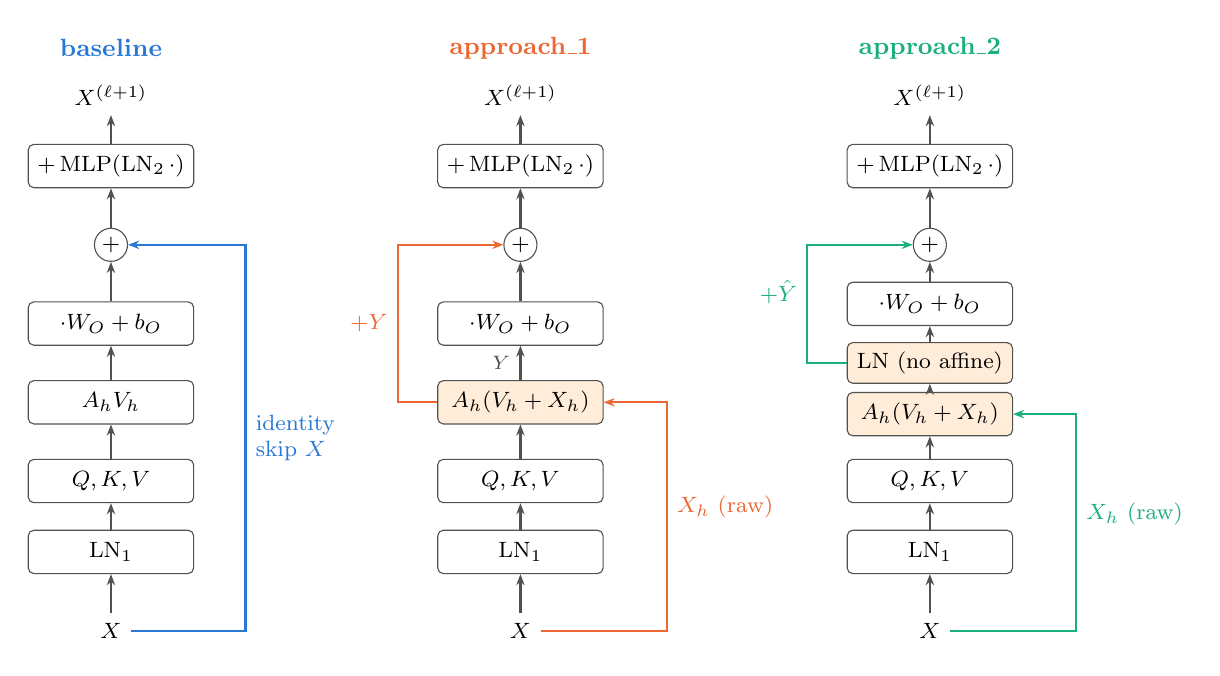
\begin{tikzpicture}[
  font=\footnotesize,
  box/.style={draw=ink2, rounded corners=2pt, minimum width=2.1cm, minimum height=0.55cm, align=center, fill=white},
  op/.style={draw=ink2, circle, inner sep=0.5pt, minimum size=0.42cm, fill=white},
  new/.style={box, fill=orange!15},
  arr/.style={-{Stealth[length=4pt]}, ink2, thick},
  skip/.style={-{Stealth[length=4pt]}, thick},
]
% ---------------- baseline ----------------
\begin{scope}[xshift=0cm]
\node[font=\small\bfseries, text=cbase] at (0,7.0) {baseline};
\node (xin) at (0,-0.4) {$X$};
\node[box] (ln) at (0,0.6) {$\mathrm{LN}_1$};
\node[box] (qkv) at (0,1.5) {$Q,K,V$};
\node[box] (att) at (0,2.5) {$A_h V_h$};
\node[box] (wo) at (0,3.5) {$\cdot W_O + b_O$};
\node[op] (add) at (0,4.5) {$+$};
\node[box] (mlp) at (0,5.5) {$+\,\mathrm{MLP}(\mathrm{LN}_2\,\cdot)$};
\node (xout) at (0,6.4) {$X^{(\ell+1)}$};
\draw[arr] (xin) -- (ln); \draw[arr] (ln) -- (qkv); \draw[arr] (qkv) -- (att);
\draw[arr] (att) -- (wo); \draw[arr] (wo) -- (add); \draw[arr] (add) -- (mlp); \draw[arr] (mlp) -- (xout);
\draw[skip, cbase] (xin.east) -- ++(1.45,0) |- node[pos=0.25, right, align=left] {identity\\skip $X$} (add.east);
\end{scope}
% ---------------- approach_1 ----------------
\begin{scope}[xshift=5.2cm]
\node[font=\small\bfseries, text=cone] at (0,7.0) {approach\_1};
\node (xin) at (0,-0.4) {$X$};
\node[box] (ln) at (0,0.6) {$\mathrm{LN}_1$};
\node[box] (qkv) at (0,1.5) {$Q,K,V$};
\node[new] (att) at (0,2.5) {$A_h(V_h + X_h)$};
\node[box] (wo) at (0,3.5) {$\cdot W_O + b_O$};
\node[op] (add) at (0,4.5) {$+$};
\node[box] (mlp) at (0,5.5) {$+\,\mathrm{MLP}(\mathrm{LN}_2\,\cdot)$};
\node (xout) at (0,6.4) {$X^{(\ell+1)}$};
\draw[arr] (xin) -- (ln); \draw[arr] (ln) -- (qkv); \draw[arr] (qkv) -- (att);
\draw[arr] (att) -- node[left, font=\scriptsize] {$Y$} (wo); \draw[arr] (wo) -- (add); \draw[arr] (add) -- (mlp); \draw[arr] (mlp) -- (xout);
\draw[skip, cone] (xin.east) -- ++(1.6,0) |- node[pos=0.27, right, align=left] {$X_h$ (raw)} (att.east);
\draw[skip, cone] (att.west) -- ++(-0.5,0) |- node[pos=0.25, left, align=right] {$+Y$} (add.west);
\end{scope}
% ---------------- approach_2 ----------------
\begin{scope}[xshift=10.4cm]
\node[font=\small\bfseries, text=ctwo] at (0,7.0) {approach\_2};
\node (xin) at (0,-0.4) {$X$};
\node[box] (ln) at (0,0.6) {$\mathrm{LN}_1$};
\node[box] (qkv) at (0,1.5) {$Q,K,V$};
\node[new] (att) at (0,2.35) {$A_h(V_h + X_h)$};
\node[new, minimum height=0.45cm] (lny) at (0,3.0) {$\mathrm{LN}$ (no affine)};
\node[box] (wo) at (0,3.75) {$\cdot W_O + b_O$};
\node[op] (add) at (0,4.5) {$+$};
\node[box] (mlp) at (0,5.5) {$+\,\mathrm{MLP}(\mathrm{LN}_2\,\cdot)$};
\node (xout) at (0,6.4) {$X^{(\ell+1)}$};
\draw[arr] (xin) -- (ln); \draw[arr] (ln) -- (qkv); \draw[arr] (qkv) -- (att);
\draw[arr] (att) -- (lny); \draw[arr] (lny) -- (wo); \draw[arr] (wo) -- (add); \draw[arr] (add) -- (mlp); \draw[arr] (mlp) -- (xout);
\draw[skip, ctwo] (xin.east) -- ++(1.6,0) |- node[pos=0.27, right, align=left] {$X_h$ (raw)} (att.east);
\draw[skip, ctwo] (lny.west) -- ++(-0.5,0) |- node[pos=0.3, left, align=right] {$+\hat Y$} (add.west);
\end{scope}
\end{tikzpicture}}
\caption{One transformer block in each variant. Highlighted boxes are the changes. In the approaches the
raw residual $X$ enters only through $X_h$ \emph{inside} the attention average. There is no
identity path from $X$ to $X^{(\ell+1)}$; the MLP skip is the only identity connection.}
\label{fig:arch}
\end{figure}

\section{Training dynamics}
\begin{figure}[H]
\centering
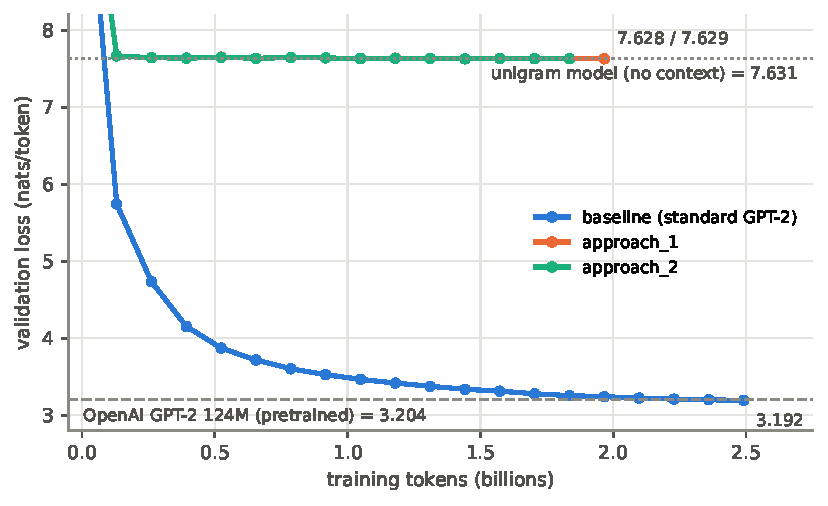
\includegraphics[width=0.82\linewidth]{figures/fig_val_loss.pdf}
\caption{Validation loss on the first 4.2M validation tokens, every 250 steps. Both reference lines are
measured on the same 4.2M tokens. Both approaches drop to the unigram line within the first eval
interval and stay there. The baseline ends level with the pretrained GPT-2 (\BaseFour{} vs.\ \RefFour{}
here; \BaseFinal{} vs.\ \RefLoss{} on the full 20M split). That is a tie, not a win, and GPT-2 is being
scored off its training distribution (WebText), so this comparison is context only.}
\label{fig:val}
\end{figure}

\begin{figure}[H]
\centering
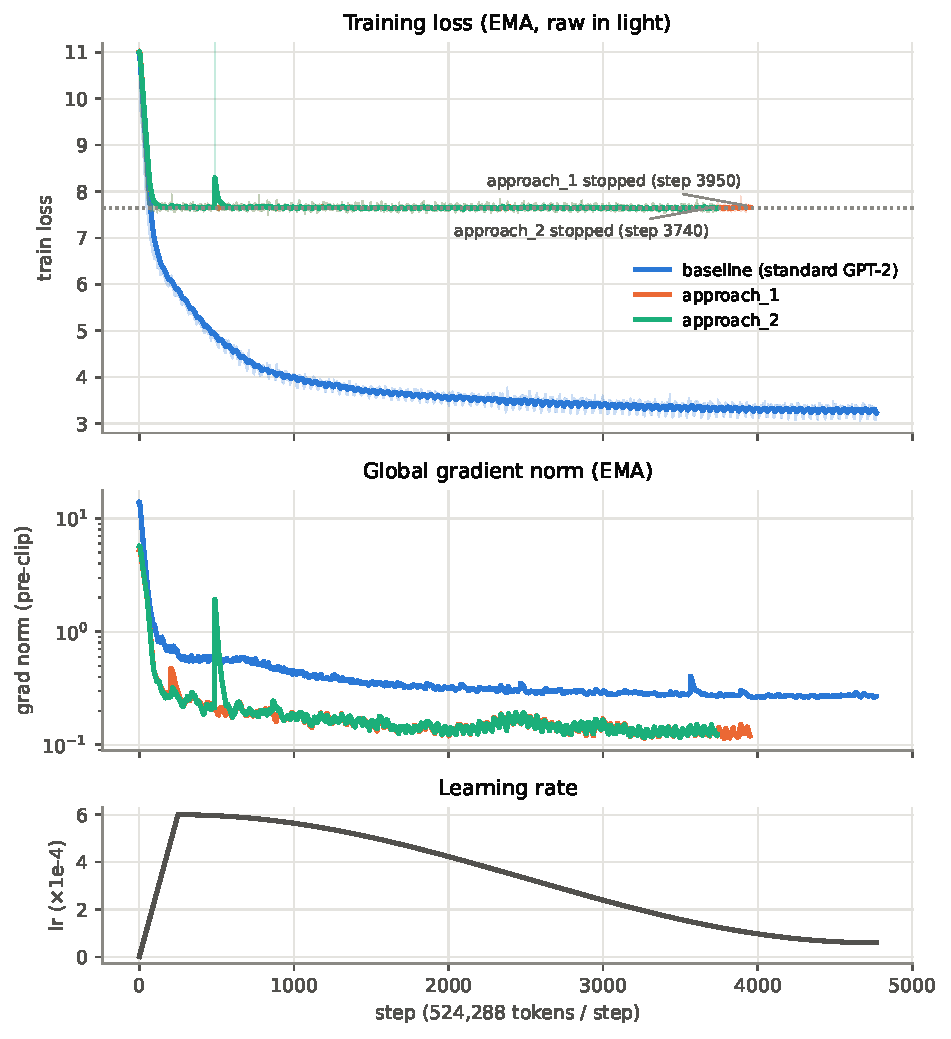
\includegraphics[width=0.75\linewidth]{figures/fig_train_dynamics.pdf}
\caption{Training loss, gradient norm and learning rate. The approaches' training loss reaches 7.65
by step $\sim$150 and then averages \OnePlateau{} (approach\_1) and \TwoPlateau{} (approach\_2) over
steps 200--3700. Their gradient norm settles about $2$--$3\times$ below the baseline's. approach\_2 has a
single spike at step 489 (loss 20.3, gradient norm 34) and returns to the same plateau within $\sim$10
steps. The plateau is an attractor.}
\label{fig:train}
\end{figure}

\begin{center}
\begin{tabular}{rrrrr}
\toprule
Step & Tokens & baseline & approach\_1 & approach\_2 \\
\midrule
\ValTable
\bottomrule
\end{tabular}
\end{center}

Observations:
\begin{itemize}
\item \textbf{Same start, early split.} All runs start at $\ln 50304 \approx 10.8$--$11.0$. The approaches
learn token frequencies (the fastest and easiest gain, from 11 to 7.65) at the same rate as the baseline,
but then stop. The baseline continues past the bigram regime ($\approx 6$) and onward.
\item \textbf{Approaches 1 and 2 are indistinguishable in loss.} Their curves overlap to within 0.002 nats.
The LayerNorm in approach\_2 changes the activation scale (Section~\ref{sec:norm}) but not what the
model can compute.
\item \textbf{Learning rate is not the issue.} The plateau persists through peak LR and through the cosine
decay. No phase of the schedule moves it.
\end{itemize}

\section{Why training collapses}
\subsection{Evidence: the models predict the unigram distribution everywhere}
\begin{figure}[H]
\centering
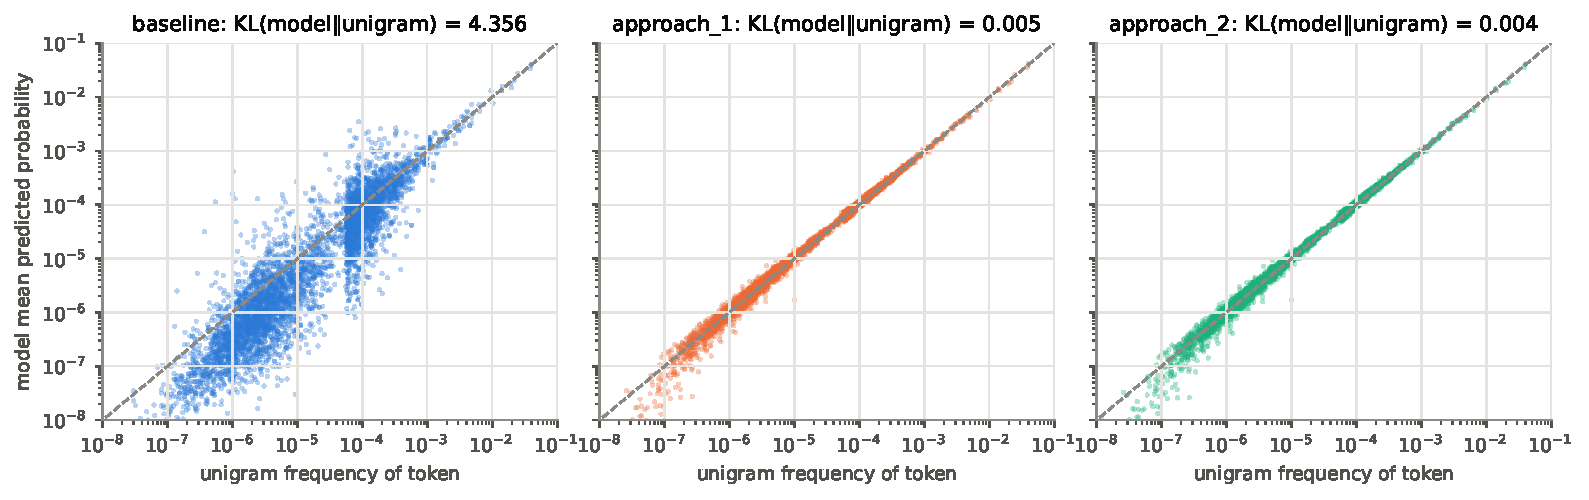
\includegraphics[width=\linewidth]{figures/fig_unigram_match.pdf}
\caption{Mean predicted probability of each token (over 8 val sequences) against its unigram frequency.
KL is averaged per position. For the approaches, every point lies on the diagonal and the
per-position KL to the unigram is $\approx$0.005 nats. Their predictions also vary across positions by
only $\sim10^{-11}$ (std of probabilities), against $\sim10^{-4}$ for the baseline. The output ignores
the input.}
\label{fig:unigram}
\end{figure}

A model whose output does not depend on the input can do no better than the token marginal, and its
loss is the unigram cross-entropy. The approaches sit at exactly this value: \OneTwenty{} and
\TwoTwenty{} against the unigram's \UniCE{} on the 20M split, and \OneFour{} and \TwoFour{} against
\UniFour{} on the 4.2M subset.

\subsection{Evidence: rank collapse of the residual stream, already at initialization}
\begin{figure}[H]
\centering
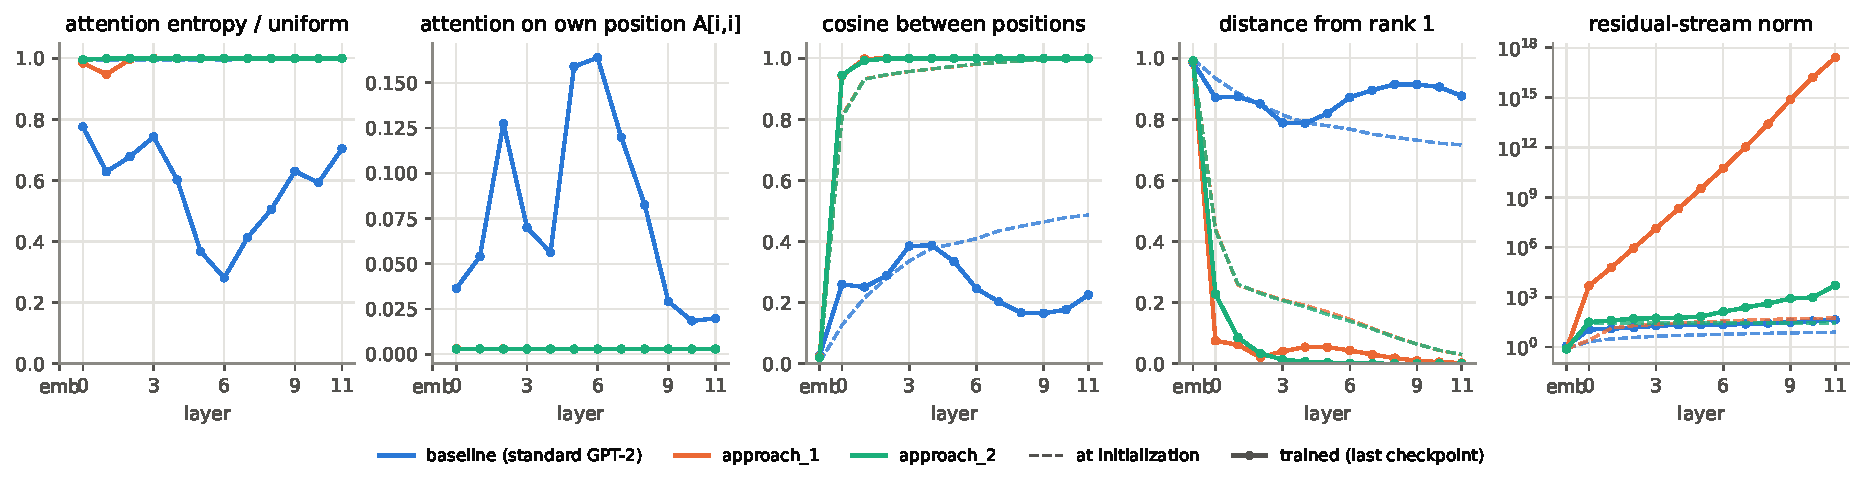
\includegraphics[width=\linewidth]{figures/fig_layer_diagnostics.pdf}
\caption{Per-layer diagnostics on 8 val sequences (positions $\ge 64$), at initialization (dashed) and at
the last checkpoint (solid; approaches at step 3000). \emph{Distance from rank 1} is
$\|X-\mathbf 1\bar x^\top\|_F/\|X\|_F$, which is 0 when every position holds the same vector.}
\label{fig:layers}
\end{figure}

Figure~\ref{fig:layers} shows the mechanism directly:
\begin{itemize}
\item \textbf{At initialization}, the approaches' residual streams already lose their per-position content.
The distance from rank 1 falls from 0.99 (embeddings) to 0.44 after layer 0 and to 0.03 after layer 11,
with cosine between positions 0.999. The baseline at initialization keeps 0.72.
\item \textbf{After training}, it is worse. The approaches reach cosine $\approx 1.000$ between positions from layer 1 on, and
distance from rank 1 of at most 0.002 at layer 11. Attention entropy equals that of uniform attention ($1.000$) in every layer except layer 0, and the
weight on a token's own position is $1/T$ on average ($0.003$). Training pushed the models
\emph{further} into collapse.
\item The baseline is the opposite. Its attention sharpens (entropy ratio 0.27--0.80), and its distance from
rank 1 rises to $\approx 0.9$.
\end{itemize}

\begin{figure}[H]
\centering
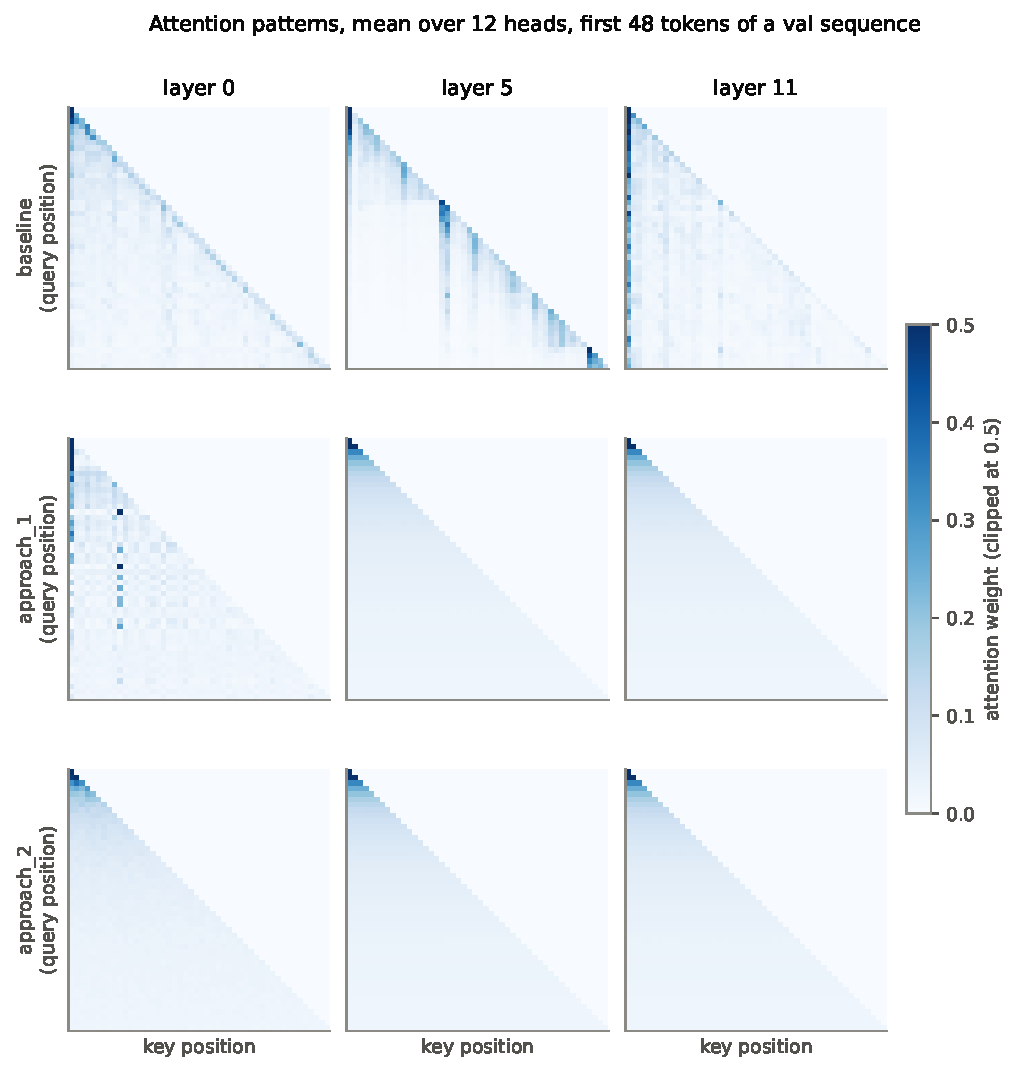
\includegraphics[width=0.66\linewidth]{figures/fig_attention_heatmaps.pdf}
\caption{Trained attention patterns (mean over heads). Baseline heads show diagonal, previous-token and
block structure. In the approaches, layers 5 and 11 are exactly uniform over the causal prefix (row $i$
is $1/(i{+}1)$, which fades with $i$). Only approach\_1's layer 0, whose input is the un-collapsed embedding,
shows any learned structure.}
\label{fig:heat}
\end{figure}

\subsection{Mechanism 1: averaging the residual causes rank collapse}
Suppose attention is uniform, $A_h = P$ with $P_{ij} = \tfrac{1}{i+1}\,[j\le i]$, which is what
initialization produces (small $Q,K$ give near-uniform softmax). The approach\_1 block then gives
\[
X' = P\,(V + X)\,(W_O + I) + b_O,\qquad X^{(\ell+1)} = X' + \mathrm{MLP}(\mathrm{LN}_2(X')).
\]
The token-mixing part is the \emph{same} averaging operator $P$ in every layer, and nothing preserves the
un-averaged $X$. After $\ell$ layers, the position-dependent content is acted on by $P^\ell$. $P$ is
row-stochastic with a single eigenvalue-1 direction (the constant vector $\mathbf 1$), so $P^\ell X$
converges to $\mathbf 1\,c^\top$: every position holds the same vector. The MLP is applied per
position and cannot restore information that is no longer present. This is the \emph{rank collapse} of
pure self-attention described by Dong, Cordonnier and Loukas (2021, ``Attention is not all you need:
pure attention loses rank doubly exponentially with depth''). In their analysis, the skip connection is
what prevents it.

\begin{figure}[H]
\centering
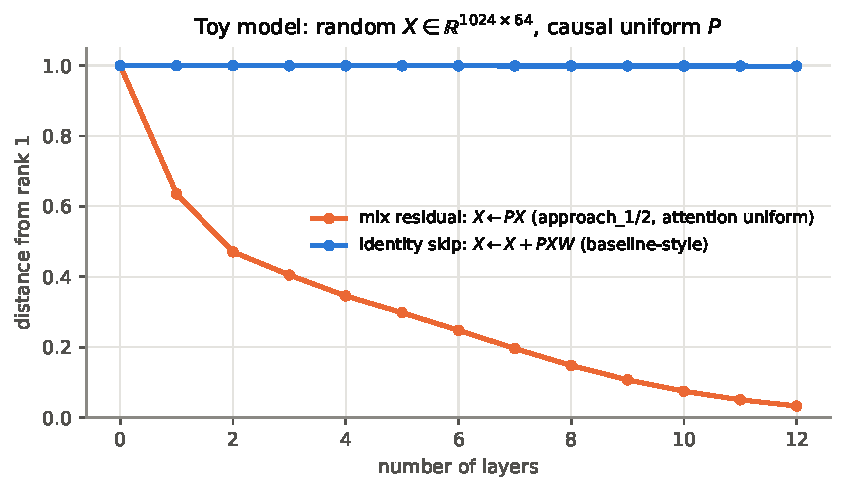
\includegraphics[width=0.72\linewidth]{figures/fig_toy_rank_collapse.pdf}
\caption{Toy model with random $X$ and uniform causal $P$. Repeatedly mixing the residual ($X\leftarrow PX$) drives it
to rank 1, reaching 0.03 after 12 layers, the same value measured in the real approach models at
initialization. With an identity skip ($X\leftarrow X+PXW$) the stream keeps its full rank.}
\label{fig:toy}
\end{figure}

In the baseline, $X^{(\ell+1)} = X + \text{(attention)} + \text{(MLP)}$, so the identity term carries every
token's own state through all 12 layers no matter what attention does. In the approaches, the only
route for $X$ is through $A_h$.

\subsection{Mechanism 2: a collapsed stream gives attention zero gradient}
\begin{prop}
If the input to a layer is identical at all positions, $X = \mathbf 1 x^\top$, then the gradient of any
loss with respect to that layer's attention logits is exactly zero, and its attention is exactly uniform.
\end{prop}
\begin{proof}
$\mathrm{LN}_1$ acts per position, so $\tilde X = \mathbf 1\tilde x^\top$ and $q_i = q$, $k_j = k$, $v_j = v$,
$x_{h,j} = x_h$ for all $i,j$. The logits $S_{ij} = q\cdot k/\sqrt{d_h}$ are constant over the causal
prefix, so $A$ is uniform. With $u_j = v_j + x_{h,j} = u$ and $g_i = \partial\mathcal L/\partial O_i$, the
softmax Jacobian gives
\[
\frac{\partial\mathcal L}{\partial S_{ij}}
= A_{ij}\Big(g_i\!\cdot u_j - \sum_{k\le i} A_{ik}\, g_i\!\cdot u_k\Big)
= A_{ij}\big(g_i\!\cdot u - g_i\!\cdot u\big) = 0. \qedhere
\]
\end{proof}

This explains why training cannot escape. Every layer from $\ell\ge 1$ receives an (almost) collapsed
input at initialization, so its $W_Q, W_K$ get (almost) no gradient toward sharper attention. Only
layer 0 sees un-collapsed embeddings and can learn structure (Figure~\ref{fig:heat}, top-left of
approach\_1). Any gain there is erased by the averaging in layers 1--11, so it cannot lower the loss.
The remaining gradient signal is fastest to reduce by fitting the unigram, which needs only a constant
output and therefore benefits from \emph{more} collapse. The optimizer drives the model deeper into the
collapsed state (distance from rank 1 from 0.03 to $<0.003$). The approach\_2 spike at step 489 shows the
state is stable: a large perturbation returns to the same loss within 10 steps.

\subsection{Mechanism 3: residual norm explosion in approach\_1}\label{sec:norm}
Once collapsed, $X = \mathbf 1 x^\top$, and approach\_1's update on the shared vector is
\[
x \;\mapsto\; \big(\mathrm{LN}_1(x)\,W_V + b_V + x\big)\,(W_O + I) + b_O + \mathrm{MLP}(\cdot)
\;=\; x\,(W_O + I) + \text{(bounded terms)}.
\]
The $V$ path reads the normalized $\mathrm{LN}_1(x)$, which is bounded, but the residual itself is carried by
the un-normalized linear map $x\mapsto x(W_O+I)$, applied 12 times. Its gain compounds geometrically:
the measured growth is \OneGrowthInit$\times$ per layer at initialization and \OneGrowth$\times$ per layer after
training, giving a residual norm of \OneNormEnd{} at layer 11 (baseline: \BaseNormEnd). Since $\mathrm{LN}_1$,
$\mathrm{LN}_2$ and $\mathrm{LN}_f$ normalize everything the network reads, the loss is unaffected; the
growth is a symptom, not the cause. approach\_2's $\mathrm{LN}(Y)$ bounds the attention output to norm
$\sqrt D\approx 27.7$, which limits the growth to \TwoGrowth$\times$ per layer (layer-11 norm \TwoNormEnd). It does not
prevent collapse, because it normalizes a vector that is already the same at every position.

\section{Conclusions and suggested fixes}
\begin{enumerate}
\item Both approaches are \textbf{untrainable as specified}. They collapse to a context-free unigram
predictor (loss \UniCE) because they remove the identity residual and route the token's own state
through the attention average. The baseline trained under identical conditions reaches \BaseFinal,
level with the pretrained GPT-2 124M (\RefLoss).
\item The failure is \textbf{present at initialization} and is a \textbf{gradient-free fixed point}, so
tuning learning rate, warmup or training length will not fix it.
\item Normalizing $Y$ (approach\_2) fixes the norm explosion but not the collapse.
\end{enumerate}
Variants that keep the idea of feeding $X_h$ into attention while avoiding the collapse:
\begin{itemize}
\item \textbf{Restore the identity skip:} $X' = X + \mathrm{Concat}_h[A_h(V_h+X_h)]W_O + b_O$. Attention can still
read the raw residual, and the token's own state is preserved.
\item \textbf{Do not mix $X_h$:} $O_h = A_h V_h + X_h$, adding the residual per position after
attention. This is equivalent to an identity skip routed through $W_O$.
\item \textbf{Gated mixing:} $X' = X + \alpha\,(\ldots)$ or $X' = (1-\alpha)X + \alpha\,\mathrm{Concat}_h[A_h X_h]$
with $\alpha$ initialized near 0, so training starts from the standard GPT-2 and the
mixing grows only if it helps.
\end{itemize}

\section*{Files in this folder}
{\small
\begin{tabularx}{\linewidth}{@{}lX@{}}
\code{report.pdf}, \code{report.tex}, \code{numbers.tex} & this report and its auto-generated numbers \\
\code{figures/} & all plots (PDF and PNG) \\
\code{data/<variant>/log.jsonl} & per-step train loss, lr, grad norm, step time; val loss every 250 steps \\
\code{data/<variant>/config.json} & run configuration \\
\code{data/<variant>/stdout.log} & console output \\
\code{data/openai\_gpt2\_124M.json} & pretrained GPT-2 val loss on the same split \\
\code{data/matched\_evals.json} & every model and the unigram on identical 4.2M and 20M val subsets \\
\code{data/collapse\_probe.json} & per-layer diagnostics at init and last checkpoint, unigram CE, KL \\
\code{data/summary.json} & final numbers \\
\end{tabularx}}

{\raggedright To reproduce:
\begin{enumerate}
\item \code{train/prepare\_fineweb.py}: download and tokenize the data;
\item \code{train/run\_chinchilla.sh}: train the three variants and evaluate pretrained GPT-2;
\item \code{train/finalize\_report.sh}: run the diagnostics (\code{analyze\_collapse.py}), the figures
(\code{make\_figures.py}) and the numbers (\code{report\_numbers.py}), then build this PDF.
\end{enumerate}
Checkpoints (1.5 GB each) are kept outside the repo, in \code{runs/chinchilla/} under
\code{/local/scratch/a/liu3170}.\par}

\end{document}
